% !TeX program = xelatex
\documentclass[a4paper,10pt]{article}

% ============================================================================
% ១. កញ្ចប់បណ្ណាល័យ និងការកំណត់ទំព័រ (Packages & Page Setup — តាមគំរូ ls_plan.tex)
% ============================================================================
\usepackage[a4paper, left=0.95cm, right=0.95cm, top=0.85cm, bottom=0.92cm, footskip=0.52cm]{geometry}
\usepackage{amsmath}
\usepackage{unicode-math}
\usepackage{fontspec}
\usepackage{longtable, array, multirow, colortbl}
\usepackage[table]{xcolor}
\usepackage{enumitem}
\usepackage{pifont}
\usepackage{fancyhdr}
\usepackage{tikz}
\usetikzlibrary{calc, arrows.meta, decorations.pathreplacing, patterns, positioning, babel}

\makeatletter
\let\@expl@@@mark@update@singlecol@structures@@\relax
\makeatother

% --- ប្រព័ន្ធស្វែងរកទីតាំងពុម្ពអក្សរស្វ័យប្រវត្តិ (Windows Local + Cloud Repo fonts/) ---
\providecommand{\NGSFindFonts}{%
  \IfFileExists{C:/Windows/Fonts/cambria.ttc}{%
    \def\NGSSysPath{C:/Windows/Fonts/}%
    \def\NGSUserPath{C:/Users/KIT/AppData/Local/Microsoft/Windows/Fonts/}%
  }{%
    \IfFileExists{./fonts/KhmerOSsiemreap.ttf}{\def\NGSSysPath{./fonts/}\def\NGSUserPath{./fonts/}}{%
    \IfFileExists{../fonts/KhmerOSsiemreap.ttf}{\def\NGSSysPath{../fonts/}\def\NGSUserPath{../fonts/}}{%
    \IfFileExists{../../fonts/KhmerOSsiemreap.ttf}{\def\NGSSysPath{../../fonts/}\def\NGSUserPath{../../fonts/}}{%
    \IfFileExists{../../../fonts/KhmerOSsiemreap.ttf}{\def\NGSSysPath{../../../fonts/}\def\NGSUserPath{../../../fonts/}}{%
    \IfFileExists{../../../../fonts/KhmerOSsiemreap.ttf}{\def\NGSSysPath{../../../../fonts/}\def\NGSUserPath{../../../../fonts/}}{%
    \IfFileExists{../../../../../fonts/KhmerOSsiemreap.ttf}{\def\NGSSysPath{../../../../../fonts/}\def\NGSUserPath{../../../../../fonts/}}{%
    \IfFileExists{../../../../../../fonts/KhmerOSsiemreap.ttf}{\def\NGSSysPath{../../../../../../fonts/}\def\NGSUserPath{../../../../../../fonts/}}{%
      \def\NGSSysPath{../../../../../../../fonts/}\def\NGSUserPath{../../../../../../../fonts/}%
    }}}}}}}%
  }%
}
\NGSFindFonts

% ============================================================================
% ២. កំណត់ពុម្ពអក្សរ (Fonts — តាមគំរូ ls_plan.tex)
% ============================================================================
\setmathfont[Path={\NGSSysPath}, FontIndex=1, Scale=1.02]{cambria.ttc}
\defaultfontfeatures{Ligatures=TeX}

\setmainfont[
  Path={\NGSUserPath},
  Extension=.ttf,
  Script=Khmer,
  BoldFont={KhmerOSsiemreap},
  BoldFeatures={FakeBold=1.8},
  ItalicFont={KhmerOSsiemreap},
  ItalicFeatures={FakeSlant=0.25},
  BoldItalicFont={KhmerOSsiemreap},
  BoldItalicFeatures={FakeBold=1.8, FakeSlant=0.25}
]{KhmerOSsiemreap}

\newfontfamily\muol[Path={\NGSUserPath}, Extension=.ttf, Script=Khmer]{KhmerOSmuollight}
\newfontfamily\Tacteing[Path={\NGSUserPath}, Extension=.TTF]{TACTENG}
\newfontfamily\TimesEn[Path={\NGSSysPath}, Extension=.ttf, BoldFont={timesbd}, ItalicFont={timesi}, BoldItalicFont={timesbi}]{times}
\newfontfamily\CalibriFont[Path={\NGSSysPath}, Extension=.ttf]{calibri}
\newfontfamily\CourierCirc[Path={\NGSSysPath}, Extension=.ttf]{cour}

\XeTeXlinebreaklocale "km"
\XeTeXlinebreakskip = 0pt plus 1pt minus 0.1pt

% ============================================================================
% ៣. ពណ៌ និងការតុបតែង (Colors & Styles)
% ============================================================================
\definecolor{stepbg}{HTML}{D9D9D9}
\definecolor{headgray}{HTML}{E6E6E6}
\definecolor{emphred}{HTML}{C00000}

\pagestyle{fancy}
\fancyhf{}
\renewcommand{\headrulewidth}{0pt}
\fancyfoot[R]{\CalibriFont\fontsize{9pt}{11pt}\selectfont\thepage}

\setlength{\parindent}{0pt}
\setlength{\parskip}{0pt}
\setlength{\tabcolsep}{4.5pt}
\setlength{\LTpre}{2pt}
\setlength{\LTpost}{2pt}

\newcolumntype{L}[1]{>{\raggedright\arraybackslash}p{#1}}
\newcolumntype{C}[1]{>{\centering\arraybackslash}p{#1}}

% ============================================================================
% ៤. ពាក្យបញ្ជាជំនួយ (Helper Macros)
% ============================================================================
\newcommand{\en}[1]{{\TimesEn #1}}
\newcommand{\enbf}[1]{{\TimesEn\bfseries #1}}
\newcommand{\khmflourish}{{\Tacteing\fontsize{15pt}{15pt}\selectfont 3}}
\newcommand{\wcirc}{{\CourierCirc\fontsize{9.5pt}{11pt}\selectfont o}}
\newcommand{\ditem}{{\fontsize{7.5pt}{10pt}\selectfont\ding{117}}\ }
\newcommand{\fiveE}[1]{\textcolor{emphred}{\CalibriFont\bfseries #1}}
\newcommand{\redsub}[1]{\textcolor{emphred}{#1}}
\newcommand{\timenote}[1]{\textcolor{emphred}{\textit{#1}}}
\newcommand{\stepheader}[1]{\multicolumn{3}{|c|}{\cellcolor{stepbg}\muol #1} \\ \hline}
\newcommand{\cfig}[1]{{\centering\vspace{3pt}#1\vspace{3pt}\par}}
\newcommand{\cnum}[1]{\mbox{\fontsize{10.5pt}{12pt}\selectfont\ding{\numexpr181+#1\relax}}}
\newcommand{\unit}[1]{\,\text{\en{#1}}}
\newcommand{\riel}{\,\text{៛}}
\newcommand{\graybox}[1]{\colorbox{headgray}{\strut #1}}

% ============================================================================
% ៥. រូបភាព TikZ ស-ខ្មៅ សម្រាប់បង្រៀនលើក្ដារខៀន និងសន្លឹកកិច្ចការ (B&W Diagrams)
% ============================================================================

% ១. E1 Engage: អន្ទាក់ភ្លេចវង់ក្រចកពេលដកភាគយកពហុធា a/(2a+3) - (a-3)/(2a+3) (ទំ.៨១)
\newcommand{\figEngageRATSixFour}{%
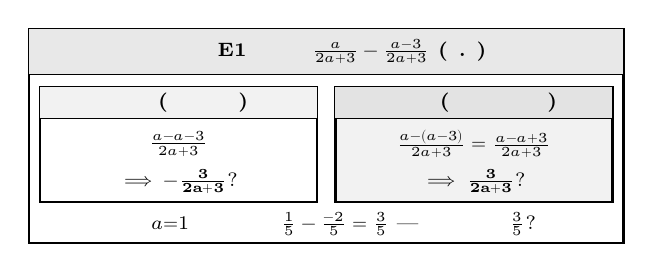
\begin{tikzpicture}[x=1cm, y=1cm, every node/.style={font=\scriptsize, text=black}]
  \draw[black, line width=0.9pt] (0,0) rectangle (7.55,2.72);
  \fill[gray!18] (0,2.14) rectangle (7.55,2.72);
  \draw[black, line width=0.6pt] (0,2.14) -- (7.55,2.14);
  \node at (3.775,2.43) {\textbf{បេសកកម្ម \en{E1}៖ គណនាផលដក $\tfrac{a}{2a + 3} - \tfrac{a - 3}{2a + 3}$ (ទំ.៨១)}};

  % Student A
  \draw[black, line width=0.8pt] (0.14,0.52) rectangle (3.66,1.98);
  \fill[gray!10] (0.14,1.58) rectangle (3.66,1.98);
  \draw[black, line width=0.5pt] (0.14,1.58) -- (3.66,1.58);
  \node at (1.90,1.78) {\textbf{សិស្ស ក (គ្មានវង់ក្រចក)}};
  \node at (1.90,1.26) {$\tfrac{a - a - 3}{2a + 3}$};
  \node at (1.90,0.78) {$\implies \mathbf{-\tfrac{3}{2a + 3}}$?};

  % Student B
  \draw[black, line width=0.95pt, fill=gray!10] (3.89,0.52) rectangle (7.41,1.98);
  \fill[gray!22] (3.89,1.58) rectangle (7.41,1.98);
  \draw[black, line width=0.55pt] (3.89,1.58) -- (7.41,1.58);
  \node at (5.65,1.78) {\textbf{សិស្ស ខ (ដាក់វង់ក្រចកការពារ)}};
  \node at (5.65,1.26) {$\tfrac{a - (a - 3)}{2a + 3} = \tfrac{a - a + 3}{2a + 3}$};
  \node at (5.65,0.78) {$\implies \mathbf{\tfrac{3}{2a + 3}}$?};

  \node at (3.775,0.24) {\textbf{តេស្ត $a{=}1$៖} កន្សោមដើមស្មើ $\tfrac{1}{5} - \tfrac{-2}{5} = \tfrac{3}{5}$ — តើចម្លើយណាស្មើ $\tfrac{3}{5}$?};
\end{tikzpicture}}

% ២. E2 Explore: បូក-ដកភាគបែងដូចគ្នា និងភាគបែងផ្ទុយ 3-x = -(x-3) (ទំ.៨១)
\newcommand{\figExploreRATSixFour}{%
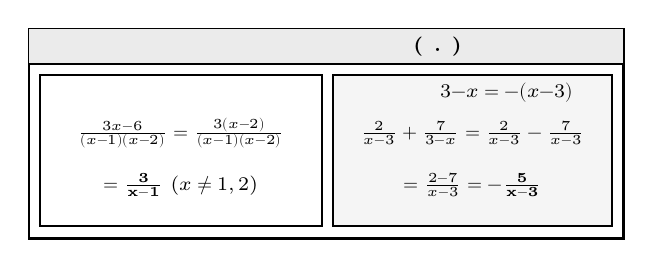
\begin{tikzpicture}[x=1cm, y=1cm, every node/.style={font=\scriptsize, text=black}]
  \draw[black, line width=0.9pt] (0,0) rectangle (7.55,2.66);
  \fill[gray!16] (0,2.22) rectangle (7.55,2.66);
  \draw[black, line width=0.6pt] (0,2.22) -- (7.55,2.22);
  \node at (3.775,2.44) {\textbf{ការសម្រួលក្រោយដក និងការប្ដូរភាគបែងផ្ទុយ (ទំ.៨១)}};

  % Left: Subtract & simplify
  \draw[black, line width=0.8pt] (0.14,0.16) rectangle (3.72,2.08);
  \node at (1.93,1.86) {\textbf{ដករួចដាក់ជាកត្តាសម្រួល}};
  \node at (1.93,1.34) {$\tfrac{3x - 6}{(x - 1)(x - 2)} = \tfrac{3(x - 2)}{(x - 1)(x - 2)}$};
  \node at (1.93,0.68) {$= \mathbf{\tfrac{3}{x - 1}}$ ($x \neq 1, 2$)};

  % Right: Opposite denominator
  \draw[black, line width=0.8pt, fill=gray!8] (3.86,0.16) rectangle (7.41,2.08);
  \node at (5.635,1.86) {\textbf{ភាគបែងផ្ទុយ $3{-}x = -(x{-}3)$}};
  \node at (5.635,1.34) {$\tfrac{2}{x - 3} + \tfrac{7}{3 - x} = \tfrac{2}{x - 3} - \tfrac{7}{x - 3}$};
  \node at (5.635,0.68) {$= \tfrac{2 - 7}{x - 3} = \mathbf{-\tfrac{5}{x - 3}}$};
\end{tikzpicture}}

% ៣. E3 Explain: វិធានបូក-ដកភាគបែងដូចគ្នា និងភាគបែងផ្ទុយ (ទំ.៨១)
\newcommand{\figRuleRATSixFour}{%
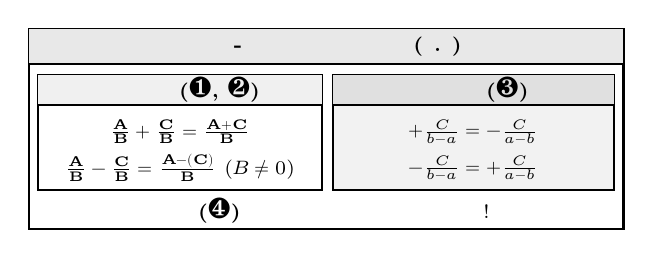
\begin{tikzpicture}[x=1cm, y=1cm, every node/.style={font=\scriptsize, text=black}]
  \draw[black, line width=0.9pt] (0,0) rectangle (7.55,2.54);
  \fill[gray!18] (0,2.10) rectangle (7.55,2.54);
  \draw[black, line width=0.6pt] (0,2.10) -- (7.55,2.10);
  \node at (3.775,2.32) {\textbf{វិធានបូក-ដកកន្សោមសនិទានមានភាគបែងដូចគ្នា (ទំ.៨១)}};

  % Left: Addition & Subtraction
  \draw[black, line width=0.8pt] (0.12,0.50) rectangle (3.72,1.96);
  \fill[gray!12] (0.12,1.58) rectangle (3.72,1.96);
  \draw[black, line width=0.55pt] (0.12,1.58) -- (3.72,1.58);
  \node at (1.92,1.77) {\textbf{ភាគបែងដូចគ្នា (\cnum{1}, \cnum{2})}};
  \node at (1.92,1.24) {$\mathbf{\tfrac{A}{B} + \tfrac{C}{B} = \tfrac{A + C}{B}}$};
  \node at (1.92,0.78) {$\mathbf{\tfrac{A}{B} - \tfrac{C}{B} = \tfrac{A - (C)}{B}}$ ($B \neq 0$)};

  % Right: Opposite Denominators
  \draw[black, line width=0.95pt, fill=gray!10] (3.86,0.50) rectangle (7.43,1.96);
  \fill[gray!24] (3.86,1.58) rectangle (7.43,1.96);
  \draw[black, line width=0.6pt] (3.86,1.58) -- (7.43,1.58);
  \node at (5.645,1.77) {\textbf{ភាគបែងផ្ទុយ (\cnum{3})}};
  \node at (5.645,1.24) {$+\tfrac{C}{b - a} = -\tfrac{C}{a - b}$};
  \node at (5.645,0.78) {$-\tfrac{C}{b - a} = +\tfrac{C}{a - b}$};

  \node at (3.775,0.24) {\textbf{ចំណាំ (\cnum{4})៖} បូកឬដកភាគយករួច ត្រូវដាក់ជាកត្តាសម្រួលបើអាច!};
\end{tikzpicture}}

% ៤. E4 Elaborate: ប្រតិបត្តិ ក, ខ (ទំ.៨១) និង #7 ឆ (ទំ.៨៦)
\newcommand{\figElaborateRATSixFour}{%
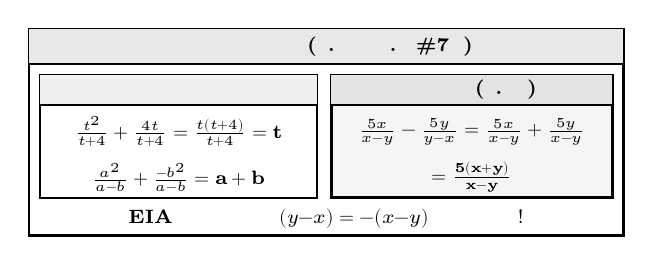
\begin{tikzpicture}[x=1cm, y=1cm, every node/.style={font=\scriptsize, text=black}]
  \draw[black, line width=0.9pt] (0,0) rectangle (7.55,2.62);
  \fill[gray!18] (0,2.18) rectangle (7.55,2.62);
  \draw[black, line width=0.6pt] (0,2.18) -- (7.55,2.18);
  \node at (3.775,2.40) {\textbf{លំហាត់ប្រតិបត្តិពង្រីក (ទំ.៨១ និង ទំ.៨៦ \en{\#7} ឆ)}};

  % Left: Practice ក & #7 ឆ
  \draw[black, line width=0.8pt] (0.14,0.48) rectangle (3.66,2.04);
  \fill[gray!12] (0.14,1.66) rectangle (3.66,2.04);
  \draw[black, line width=0.55pt] (0.14,1.66) -- (3.66,1.66);
  \node at (1.90,1.85) {\textbf{បូករួចសម្រួលកត្តារួម}};
  \node at (1.90,1.32) {$\tfrac{t^2}{t+4} + \tfrac{4t}{t+4} = \tfrac{t(t+4)}{t+4} = \mathbf{t}$};
  \node at (1.90,0.74) {$\tfrac{a^2}{a-b} + \tfrac{-b^2}{a-b} = \mathbf{a + b}$};

  % Right: Practice ខ
  \draw[black, line width=0.95pt, fill=gray!8] (3.84,0.48) rectangle (7.41,2.04);
  \fill[gray!22] (3.84,1.66) rectangle (7.41,2.04);
  \draw[black, line width=0.6pt] (3.84,1.66) -- (7.41,1.66);
  \node at (5.625,1.85) {\textbf{ភាគបែងផ្ទុយ (ទំ.៨១ ខ)}};
  \node at (5.625,1.32) {$\tfrac{5x}{x - y} - \tfrac{5y}{y - x} = \tfrac{5x}{x - y} + \tfrac{5y}{x - y}$};
  \node at (5.625,0.74) {$= \mathbf{\tfrac{5(x + y)}{x - y}}$};

  \node at (3.775,0.22) {\textbf{\en{EIA}៖} ដកជួបភាគបែងផ្ទុយ $(y{-}x) = -(x{-}y)$ ក្លាយជាសញ្ញាបូក!};
\end{tikzpicture}}

% ៥. E5 Evaluate: ជម្រើសវិនិច្ឆ័យ A-D សម្រាប់ 2x/(x-4) - (x+4)/(x-4)
\newcommand{\figExitRATSixFour}{%
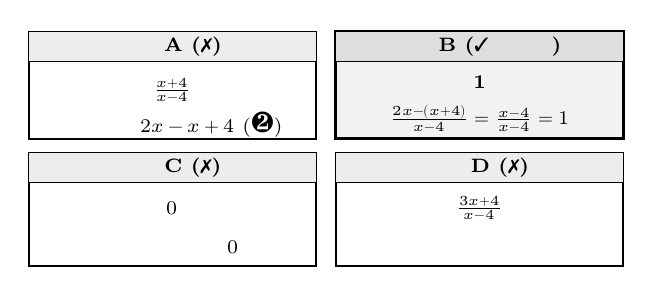
\begin{tikzpicture}[x=1cm, y=1cm, every node/.style={font=\scriptsize, text=black}]
  % Choice A
  \draw[black, line width=0.8pt] (0,1.62) rectangle (3.65,2.98);
  \fill[gray!14] (0,2.60) rectangle (3.65,2.98);
  \draw[black, line width=0.5pt] (0,2.60) -- (3.65,2.60);
  \node at (1.825,2.79) {\textbf{ជម្រើស \en{A} (\ding{55})}};
  \node at (1.825,2.24) {$\tfrac{x + 4}{x - 4}$};
  \node at (1.825,1.80) {ភ្លេចវង់ក្រចក $2x - x + 4$ (\cnum{2})};

  % Choice B (Correct)
  \draw[black, line width=1.0pt, fill=gray!10] (3.90,1.62) rectangle (7.55,2.98);
  \fill[gray!26] (3.90,2.60) rectangle (7.55,2.98);
  \draw[black, line width=0.55pt] (3.90,2.60) -- (7.55,2.60);
  \node at (5.725,2.79) {\textbf{ជម្រើស \en{B} (\ding{51} ត្រឹមត្រូវ)}};
  \node at (5.725,2.34) {$\mathbf{1}$};
  \node at (5.725,1.88) {$\tfrac{2x-(x+4)}{x-4} = \tfrac{x-4}{x-4} = 1$};

  % Choice C
  \draw[black, line width=0.8pt] (0,0) rectangle (3.65,1.44);
  \fill[gray!14] (0,1.06) rectangle (3.65,1.44);
  \draw[black, line width=0.5pt] (0,1.06) -- (3.65,1.06);
  \node at (1.825,1.25) {\textbf{ជម្រើស \en{C} (\ding{55})}};
  \node at (1.825,0.74) {$0$};
  \node at (1.825,0.24) {ច្រឡំសម្រួលដូចគ្នាបាន $0$};

  % Choice D
  \draw[black, line width=0.8pt] (3.90,0) rectangle (7.55,1.44);
  \fill[gray!14] (3.90,1.06) rectangle (7.55,1.44);
  \draw[black, line width=0.5pt] (3.90,1.06) -- (7.55,1.06);
  \node at (5.725,1.25) {\textbf{ជម្រើស \en{D} (\ding{55})}};
  \node at (5.725,0.74) {$\tfrac{3x + 4}{x - 4}$};
  \node at (5.725,0.24) {ច្រឡំបូកជំនួសឱ្យដក};
\end{tikzpicture}}

% ============================================================================
% ៦. ចាប់ផ្ដើមឯកសារ (Document Body)
% ============================================================================
\begin{document}
\fontsize{10pt}{15.2pt}\selectfont

% --- ក្បាលរដ្ឋបាល (Administrative Header) ---
\begin{center}
  {\muol\fontsize{11pt}{16pt}\selectfont ព្រះរាជាណាចក្រកម្ពុជា}\\[2pt]
  {\muol\fontsize{11pt}{16pt}\selectfont ជាតិ សាសនា ព្រះមហាក្សត្រ}\\[-2pt]
  \khmflourish
\end{center}
\vspace{-4pt}

{\muol\fontsize{10pt}{15pt}\selectfont
មន្ទីរអប់រំ យុវជន និងកីឡា ខេត្តកំពង់ធំ\\
ការិយាល័យអប់រំ យុវជន និងកីឡា ស្រុកកំពង់ស្វាយ\\
អនុវិទ្យាល័យព្រះក្រសាំង}

\vspace{2pt}
\begin{center}
  {\muol\fontsize{12pt}{18pt}\selectfont កិច្ចតែងការបង្រៀន}
\end{center}
\vspace{1pt}

% --- ព័ត៌មានទូទៅ (General Metadata) ---
\begin{tabular}{@{}p{1.85cm}p{3.25cm}@{\hspace{4pt}:\hspace{6pt}}p{12.65cm}@{}}
  & - \quad មុខវិជ្ជា          & គណិតវិទ្យា ថ្នាក់ទី៨ (ពីជគណិត) \\
  & - \quad ចំណងជើងមេរៀន & មេរៀនទី៦៖ កន្សោមសនិទាន \\
  & - \quad ចំណងជើងរង      & ៥.១ វិធីបូកនិងវិធីដកកន្សោមសនិទានមានភាគបែងដូចគ្នា \\
  & - \quad រយៈពេល             & ១ ម៉ោងសិក្សា (៥០ នាទី) \\
  & - \quad បង្រៀនដោយ         & ហុក ប៊ុនថែន \\
  & - \quad កាលបរិច្ឆេទ        & ថ្ងៃព្រហស្បតិ៍ ទី១៧ ខែធ្នូ ឆ្នាំ២០២៦ \\
\end{tabular}

\vspace{4pt}

% --- I. វត្ថុបំណង ---
{\muol\enbf{I.} វត្ថុបំណង}\par\vspace{2pt}
\begin{tabular}{@{}p{0.55cm}p{2.55cm}@{\hspace{2pt}:\hspace{6pt}}L{15.4cm}@{}}
  & \wcirc វិជ្ជាសម្បទា   & សិស្សប្រាប់បាននូវវិធានបូកនិងដកកន្សោមសនិទានមានភាគបែងដូចគ្នា $\tfrac{A}{B} \pm \tfrac{C}{B} = \tfrac{A \pm C}{B}$ ($B \neq 0$) និងករណីភាគបែងផ្ទុយគ្នាបានត្រឹមត្រូវ (ទំ.៨១) ។ \\[2pt]
  & \wcirc បំណិនសម្បទា & សិស្សគណនាផលបូកនិងផលដកកន្សោមសនិទានមានភាគបែងដូចគ្នា ឬផ្ទុយគ្នា រួចសម្រួលលទ្ធផលលើសន្លឹកកិច្ចការបានត្រឹមត្រូវ ។ \\[2pt]
  & \wcirc ចរិយាសម្បទា  & សិស្សមានទម្លាប់ដាក់វង់ក្រចកការពារភាគយកទី ២ ពេលធ្វើប្រមាណវិធីដក និងពិនិត្យសញ្ញាប្រកបដោយភាពម៉ត់ចត់ ។ \\
\end{tabular}

\vspace{3pt}

% --- II. សម្ភារៈឧបទេស (Zero-LCD & Fill-In Worksheet Context) ---
{\muol\enbf{II.} សម្ភារៈឧបទេស}\par\vspace{2pt}
\hspace*{0.55cm}$\bullet$ សៀវភៅសិក្សាគោលថ្នាក់ទី៨ (ទំ.៨១, ៨៦) ក្ដារខៀន ដីស/ហ្វឺត បន្ទាត់ត្រង់ និង\textbf{សន្លឹកកិច្ចការសិស្សបំពេញចន្លោះ ស-ខ្មៅ} (កូដ \en{RAT64} ទំព័រ ១--២ សម្រាប់សិស្ស និងទំព័រ ៣ ប្លង់ក្ដារខៀន/ចម្លើយគ្រូ — គ្មានប្រើ \en{LCD})

\vspace{3pt}

% --- III. វិធីសាស្រ្តបង្រៀន ---
{\muol\enbf{III.} វិធីសាស្រ្តបង្រៀន}\par\vspace{2pt}
\begin{tabular}{@{}p{0.55cm}p{2.55cm}@{\hspace{2pt}:\hspace{6pt}}L{15.4cm}@{}}
  & $\bullet$ គោលវិធី      & សិស្សមជ្ឈមណ្ឌល (សន្លឹកកិច្ចការបំពេញចន្លោះជាគោល + ការពិភាក្សាជាក្រុមតូច ៣ នាក់) \\
  & $\bullet$ យុទ្ធវិធីបង្រៀន & គំរូស្ថាបនានិយម \en{5Es} រួមបញ្ចូល \textit{ការវិភាគលំហាត់គំរូខុស (\en{Erroneous Examples})} និង \textit{វង់ក្រចកការពារផលដក} \\
\end{tabular}

\vspace{4pt}

% --- IV. ដំណើរការបង្រៀន (50-Minute 5E Flow) ---
{\muol\enbf{IV.} ដំណើរការបង្រៀន}\par\vspace{1pt}

\renewcommand{\arraystretch}{1.15}
\begin{longtable}{|L{5.50cm}|L{7.90cm}|L{4.80cm}|}
\hline
\multicolumn{1}{|c|}{\cellcolor{headgray}\muol សកម្មភាពគ្រូ} &
\multicolumn{1}{c|}{\cellcolor{headgray}\muol ខ្លឹមសារមេរៀន} &
\multicolumn{1}{c|}{\cellcolor{headgray}\muol សកម្មភាពសិស្ស} \\[2pt]
\hline
\endfirsthead

\hline
\multicolumn{1}{|c|}{\cellcolor{headgray}\muol សកម្មភាពគ្រូ} &
\multicolumn{1}{c|}{\cellcolor{headgray}\muol ខ្លឹមសារមេរៀន} &
\multicolumn{1}{c|}{\cellcolor{headgray}\muol សកម្មភាពសិស្ស} \\[2pt]
\hline
\endhead

\hline
\endfoot

% ==================== ជំហានទី១ (2min) ====================
\stepheader{ជំហានទី១ \enbf{(}រដ្ឋបាលថ្នាក់\enbf{)}}
$\bullet$ ពិនិត្យវត្តមាន អនាម័យ និងសណ្ដាប់ធ្នាប់ថ្នាក់រៀន \par
$\bullet$ រៀបចំក្រុមតូច ៣ នាក់ និងចែក\textbf{សន្លឹកកិច្ចការសិស្ស} (\en{RAT64} ទំព័រ ១–២)
&
$\bullet$ រដ្ឋបាលថ្នាក់ អនាម័យ និងវិន័យសិក្សា \par
$\bullet$ ចែកសន្លឹកកិច្ចការម្នាក់ ១ សន្លឹក សម្រាប់បំពេញតាមដំណាក់កាល \en{E1--E5}
&
$\circ$ ប្រធានថ្នាក់រាយការណ៍វត្តមានសិស្ស \par
$\circ$ ទទួលសន្លឹកកិច្ចការ សរសេរឈ្មោះ និងអង្គុយតាមក្រុម ៣ នាក់ \\
\hline

% ==================== ជំហានទី២ (9min: កំណែ ≤3m + រំលឹក 3m + E1 3m) ====================
\stepheader{ជំហានទី២ \enbf{(}កិច្ចការផ្ទះ \enbf{+} ទំនាក់ទំនងមេរៀនថ្មី\enbf{)}}
\ditem \textbf{កំណែកិច្ចការផ្ទះ (\enbf{$\le$ 3 min})} \par
$\bullet$ ហៅសិស្ស ២ នាក់ឡើងកែលំហាត់ទំ.៨៦ \en{\#6} ក, ខ និង \en{\#6} ឈ, ដ លើក្ដារខៀន
&
\hspace*{0.15cm}\redsub{កំណែកិច្ចការផ្ទះ (ទំ.៨៦ លេខ ៦ ក, ខ, ង, ឈ, ដ)} \par
$\bullet$ \textbf{\en{\#6} ក, ខ៖} ក) $\tfrac{-24x^5y^3}{30x^5y^4} = \mathbf{-\tfrac{4}{5y}}$; \quad ខ) $\tfrac{4x}{3y}\cdot\tfrac{15x^2y^3}{4xy} = \mathbf{5x^2y}$ \par
$\bullet$ \textbf{\en{\#6} ង, ឈ, ដ៖} ង) $\mathbf{b(b + 3)}$; \quad ឈ) $\mathbf{-(a + 7)}$; \quad ដ) $\mathbf{\tfrac{b - 4}{b - 3}}$
&
$\circ$ ផ្ទៀងចម្លើយ និងកែតម្រូវចូលសៀវភៅកិច្ចការផ្ទះ \\[3pt]

\ditem \textbf{រំលឹកមេរៀនទាក់ទង (\enbf{3min})} \par
$\bullet$ សួរ៖ «តើគេបូកប្រភាគ $\tfrac{3}{11} + \tfrac{5}{11}$ ដោយវិធីណា? ចុះលុបវង់ក្រចក $a - (a - 3)$ បានអ្វី?»
&
\hspace*{0.15cm}\redsub{រំលឹកការបូកប្រភាគភាគបែងដូចគ្នា និងការលុបវង់ក្រចក} \par
$\bullet$ បូកប្រភាគ៖ $\tfrac{3}{11} + \tfrac{5}{11} = \tfrac{3 + 5}{11} = \tfrac{8}{11}$ (បូកភាគយក រក្សាភាគបែងដដែល) \par
$\bullet$ លុបវង់ក្រចក៖ $a - (a - 3) = a - a + 3 = \mathbf{3}$ (សញ្ញាដកមុខវង់ក្រចកប្ដូរសញ្ញាតួខាងក្នុង!)
&
$\circ$ ឆ្លើយ៖ «បូកតែភាគយក ហើយលុបវង់ក្រចកបាន $+3$!» \\[3pt]

\fiveE{E1 - Engage (3min)} \timenote{(កុំទាន់ផ្តល់ចម្លើយ)} \par
\ditem \textbf{បេសកកម្មអន្ទាក់វង់ក្រចកពេលដកភាគយក (សន្លឹកកិច្ចការ \en{E1})} \par
$\bullet$ ឱ្យសិស្សអានប្រអប់ \en{E1} ពិនិត្យផលដក $\dfrac{a}{2a + 3} - \dfrac{a - 3}{2a + 3}$ (ទំ.៨១) ដោយជំនួស $a = 1$
&
\redsub{បេសកកម្ម \en{E1}៖ គណនា $\dfrac{a}{2a + 3} - \dfrac{a - 3}{2a + 3}$ តាមវិធីណាទើបត្រូវ? (ទំ.៨១)} \par
$\bullet$ \textbf{សិស្ស ក} សរសេរគ្មានវង់ក្រចក $\dfrac{a - a - 3}{2a + 3} = -\dfrac{3}{2a + 3}$! \par
$\bullet$ \textbf{សិស្ស ខ} ដាក់វង់ក្រចកការពារ $\dfrac{a - (a - 3)}{2a + 3} = \dfrac{3}{2a + 3}$! តេស្ត $a = 1$ មើល៍!
&
$\circ$ ជំនួស $a = 1$ ពិភាក្សាជាគូ និងគូស \ding{51} ក្នុងប្រអប់ \en{E1} \\[3pt]

&
\cfig{\figEngageRATSixFour}
& \\
\hline

% ==================== ជំហានទី៣ (17min: E2 11m + E3 6m) ====================
\stepheader{ជំហានទី៣ \enbf{(}ខ្លឹមសារមេរៀនថ្មី\enbf{)}}
\fiveE{E2 - Explore (11min)} \par
$\bullet$ សរសេរចំណងជើងរង \textbf{៥. វិធីបូកនិងវិធីដកកន្សោមសនិទាន — ៥.១ ករណីមានភាគបែងដូចគ្នា} \par
\ditem \textbf{សកម្មភាព ១៖ ភាគបែងដូចគ្នា និងការសម្រួលចម្លើយ (ទំ.៨១, \enbf{5min}, \en{E2-A})} \par
$\bullet$ ឱ្យសិស្សបំពេញឧទាហរណ៍ ក, ខ, គ (ទំ.៨១) លើ \en{E2-A}
&
៥.១ ករណីមានភាគបែងដូចគ្នា (ទំ.៨១) \par
$\bullet$ \textbf{ឧទាហរណ៍ ក, ខ៖} ក) $\dfrac{5}{a} + \dfrac{7}{a} = \mathbf{\dfrac{12}{a}}$; \quad ខ) $\dfrac{3y - 2}{y - 5} + \dfrac{8y + 7}{y - 5} = \mathbf{\dfrac{11y + 5}{y - 5}}$ \par
$\bullet$ \textbf{ឧទាហរណ៍ គ៖} $\dfrac{3x}{(x-1)(x-2)} - \dfrac{6}{(x-1)(x-2)} = \dfrac{3(x-2)}{(x-1)(x-2)} = \mathbf{\dfrac{3}{x - 1}}$
&
$\circ$ បូក-ដកភាគយក និងសម្រួលកត្តារួមលើ \en{E2-A} \\[3pt]

\ditem \textbf{សកម្មភាព ២៖ ភាគបែងផ្ទុយ $3 - x = -(x - 3)$ និងដកពហុធា (ទំ.៨១, \enbf{6min}, \en{E2-B})} \par
$\bullet$ ឱ្យសិស្សបំពេញលំហាត់គំរូ ក និង ខ (ទំ.៨១) លើ \en{E2-B}
&
ការប្ដូរភាគបែងផ្ទុយ និងការដកពហុធា (ទំ.៨១) \par
$\bullet$ \textbf{គំរូ ក៖} $\dfrac{2}{x - 3} + \dfrac{7}{3 - x} = \dfrac{2}{x - 3} - \dfrac{7}{x - 3} = \dfrac{2 - 7}{x - 3} = \mathbf{-\dfrac{5}{x - 3}}$ \par
$\bullet$ \textbf{គំរូ ខ៖} $\dfrac{a}{2a + 3} - \dfrac{a - 3}{2a + 3} = \dfrac{a - (a - 3)}{2a + 3} = \dfrac{a - a + 3}{2a + 3} = \mathbf{\dfrac{3}{2a + 3}}$
&
$\circ$ ប្ដូរភាគបែងផ្ទុយ និងប្រើវង់ក្រចកការពារលើ \en{E2-B} \\[3pt]

&
\cfig{\figExploreRATSixFour}
& \\[3pt]

% --- E3 Explain (6min) ---
\fiveE{E3 - Explain (6min)} \par
$\bullet$ ដឹកនាំសិស្សសង្ខេបវិធានបូក-ដកកន្សោមសនិទានមានភាគបែងដូចគ្នា (ទំ.៨១)
&
$\bullet$ \textbf{ជាទូទៅ (ទំ.៨១)៖} ចំពោះកន្សោមសនិទានមានភាគបែងដូចគ្នា ($B \neq 0$) គេបូកឬដកភាគយក ហើយរក្សាភាគបែងទុកដដែល៖ \par
\hspace*{0.15cm}– រូបមន្ត៖ $\graybox{$\dfrac{A}{B} + \dfrac{C}{B} = \dfrac{A + C}{B}$}$ \ និង \ $\graybox{$\dfrac{A}{B} - \dfrac{C}{B} = \dfrac{A - (C)}{B}$}$ ($B \neq 0$)
&
$\circ$ បំពេញប្រអប់វិធានជាទូទៅលើសន្លឹកកិច្ចការ \en{E3} \\[3pt]

$\bullet$ ភ្ជាប់\textbf{ធនាគារហេតុផល \cnum{1}--\cnum{4}} លើក្ដារខៀន និងសន្លឹកកិច្ចការ
&
\textbf{ធនាគារហេតុផល (\en{Warrant Bank})៖} \par
\cnum{1} \textbf{រក្សាភាគបែងដដែល៖} បូកឬដកតែភាគយក ហាមបូកឬដកភាគបែងនឹងភាគបែង \par
\cnum{2} \textbf{វង់ក្រចកការពារផលដក៖} ត្រូវដាក់វង់ក្រចក $A - (C)$ ជានិច្ចពេលដកពហុធា
&
$\circ$ ផ្ទៀងលេខកូដ \cnum{1}--\cnum{2} លើសន្លឹកកិច្ចការ \\[3pt]

&
\cnum{3} \textbf{ប្ដូរភាគបែងផ្ទុយ៖} ដោយ $b - a = -(a - b)$ គេបាន $+\tfrac{C}{b-a} = -\tfrac{C}{a-b}$ និង $-\tfrac{C}{b-a} = +\tfrac{C}{a-b}$
&
$\circ$ ផ្ទៀងលេខកូដ \cnum{3} លើសន្លឹកកិច្ចការ \\[3pt]

&
\cnum{4} \textbf{សម្រួលលទ្ធផលចុងក្រោយ៖} ក្រោយបង្រួមភាគយករួច ត្រូវដាក់ជាកត្តាសម្រួលបើអាច
&
$\circ$ ផ្ទៀងលេខកូដ \cnum{4} លើសន្លឹកកិច្ចការ \\[3pt]

&
\cfig{\figRuleRATSixFour}
& \\
\hline

% ==================== ជំហានទី៤ (20min: E4 10m + E5 10m) ====================
\stepheader{ជំហានទី៤ \enbf{(}ពង្រីកចំណេះដឹង\enbf{)}}
\fiveE{E4 - Elaborate (10min)} \par
\ditem \textbf{ប្រតិបត្តិ ក, ខ (ទំ.៨១) និងលំហាត់ ទំ.៨៦ \en{\#7} ឆ} \par
$\bullet$ ឱ្យសិស្សដោះស្រាយប្រតិបត្តិ ក, ខ (ទំ.៨១) និង ទំ.៨៦ \en{\#7} ឆ លើ \en{E4}
&
\textbf{លំហាត់ប្រតិបត្តិពង្រីក (ទំ.៨១ និង ទំ.៨៦)៖} \par\vspace{2pt}
$\bullet$ \textbf{១) ប្រតិបត្តិ ក និង \en{\#7} ឆ៖} ក) $\dfrac{t^2}{t+4} + \dfrac{4t}{t+4} = \graybox{$t$}$;\quad \en{\#7} ឆ) $\dfrac{a^2}{a-b} + \dfrac{-b^2}{a-b} = \graybox{$a + b$}$ \par\vspace{3pt}
$\bullet$ \textbf{២) ប្រតិបត្តិ ខ (ទំ.៨១)៖} $\dfrac{5x}{x - y} - \dfrac{5y}{y - x} = \dfrac{5x}{x - y} + \dfrac{5y}{x - y} = \graybox{$\dfrac{5(x + y)}{x - y}$}$
&
$\circ$ ប្ដូរសញ្ញាភាគបែងផ្ទុយ បូកភាគយក និងសម្រួលលើ \en{E4} \\[3pt]

&
\cfig{\figElaborateRATSixFour}
& \\[3pt]

$\bullet$ សួរសំណួរឆ្លុះបញ្ចាំង \textbf{\en{EIA Looking-Back}} (\enbf{1min})
&
\textbf{\en{EIA Looking-Back}៖} «ក្នុងប្រតិបត្តិ ខ) $\dfrac{5x}{x - y} - \dfrac{5y}{y - x}$ ហេតុអ្វីសញ្ញាដកកណ្ដាលក្លាយជាសញ្ញាបូក ហើយមិនអាចសម្រួល $(x+y)$ នឹង $(x-y)$?» ($\to$ ព្រោះ $y - x = -(x - y)$ ដកជួបដកបានបូក \cnum{3} ហើយ $(x+y) \neq (x-y)$!)
&
$\circ$ ពន្យល់ពីការប្ដូរសញ្ញា $-(y-x) = x-y$ និងកត្តាខុសគ្នា \\[3pt]

% --- E5 Evaluate (10min) ---
\fiveE{E5 - Evaluate (10min)} \par
\ditem \textbf{ប្រតិបត្តិជាក្រុមតូច ៣ នាក់ (\enbf{4min}, សន្លឹកកិច្ចការ \en{E5})} \par
$\bullet$ ឱ្យសិស្សដោះស្រាយលំហាត់ ទំ.៨៦ \en{\#7} ក, គ, ង
&
\textbf{លំហាត់ប្រតិបត្តិ (ទំ.៨៦ លេខ ៧ ក, គ, ង)៖} \par\vspace{2pt}
$\bullet$ \textbf{១) \en{\#7} ក និង គ៖} ក) $\dfrac{12a}{7} + \dfrac{2a}{7} = \dfrac{14a}{7} = \mathbf{2a}$; \quad គ) $\dfrac{x}{x - 1} + \dfrac{1}{x - 1} = \mathbf{\dfrac{x + 1}{x - 1}}$ \par\vspace{3pt}
$\bullet$ \textbf{២) \en{\#7} ង៖} $\dfrac{6x}{x + y} + \dfrac{6y}{x + y} = \dfrac{6x + 6y}{x + y} = \dfrac{6(x + y)}{x + y} = \mathbf{6}$
&
$\circ$ សហការគ្នាបូកភាគយក និងសម្រួលកត្តារួមលើ \en{E5} \\[3pt]

$\bullet$ ឱ្យក្រុមសិស្សផ្ទៀងផ្ទាត់និងបិទ\textbf{បេសកកម្ម \en{E1}} (\enbf{2min})
&
$\bullet$ \textbf{បិទបេសកកម្ម \en{E1}៖} សិស្ស ខ ត្រឹមត្រូវ! ចំពោះ $a=1$ បាន $\dfrac{3}{2(1)+3} = \dfrac{3}{5}$ ត្រូវនឹងកន្សោមដើម (\ding{51})!
&
$\circ$ បិទបេសកកម្ម \en{E1} ឃើញសិស្ស ខ ត្រឹមត្រូវ \\[3pt]

\ditem \textbf{សំណួរវិនិច្ឆ័យ \en{A--D} និងសំបុត្រចេញ (\enbf{4min})} \par
$\bullet$ ឱ្យសិស្សគូសរង្វង់ជម្រើសត្រូវលើសន្លឹកកិច្ចការ
&
\centering\textbf{សំណួរវិនិច្ឆ័យ \en{A--D}៖ គណនាផលដក $\dfrac{2x}{x - 4} - \dfrac{x + 4}{x - 4}$}\par\vspace{4pt}
\textbf{\en{A.}} $\dfrac{x + 4}{x - 4}$ \quad
\textbf{\en{B.}} $1$ \quad
\textbf{\en{C.}} $0$ \quad
\textbf{\en{D.}} $\dfrac{3x + 4}{x - 4}$
&
$\circ$ គណនាផលដកលើសន្លឹកកិច្ចការ \\[3pt]

$\bullet$ ឱ្យសិស្សលើកម្រាមដៃ ១--៤ បង្ហាញចម្លើយព្រមគ្នា
&
\centering{\itshape (កត់សម្គាល់៖ ដាក់វង់ក្រចកការពារភាគយកទី ២ មុននឹងលុបវង់ក្រចក)}
&
$\circ$ លើកម្រាមដៃ ២ (\textbf{ជម្រើស \en{B}៖} $1$) \\[3pt]

&
\cfig{\figExitRATSixFour}
& \\[3pt]

$\bullet$ បញ្ជាក់ចម្លើយត្រូវ (\textbf{ជម្រើស \en{B}}) និងឱ្យបំពេញសំបុត្រចេញ ៦០ វិនាទី
&
$\bullet$ \textbf{សំបុត្រចេញ (ទំ.៨៦ \en{\#7} ជ)៖} គណនា $\dfrac{a}{2a - 2b} - \dfrac{b}{2a - 2b} = \dfrac{a - b}{2(a - b)} = \mathbf{\dfrac{1}{2}}$ ។
&
$\circ$ បំពេញសំបុត្រចេញលើសន្លឹកកិច្ចការមុនបញ្ចប់ម៉ោង \\
\hline

% ==================== ជំហានទី៥ (≤2min) ====================
\stepheader{ជំហានទី៥ \enbf{(}កិច្ចការផ្ទះ \enbf{+} បណ្ដាំផ្ញើ\enbf{)}}
\timenote{ចំណាយពេលឱ្យតិចបំផុតកុំឱ្យលើស 2min} \par
$\bullet$ ណែនាំប្រអប់កិច្ចការផ្ទះលើសន្លឹកកិច្ចការទំព័រ ២ (ទំ.៨៦ លេខ ៧)
&
\centering\textbf{កិច្ចការផ្ទះ (សៀវភៅគោល ទំ.៨៦ លេខ ៧ ខ, ឃ, ច, ឈ)}\par\raggedright
$\bullet$ \textbf{១) ទំ.៨៦ \en{\#7} ខ, ឃ៖} គណនា $\dfrac{y}{14} - \dfrac{3y}{14}$ និង $\dfrac{y}{b + 6} + \dfrac{2y}{b + 6}$ ។ \par
$\bullet$ \textbf{២) ទំ.៨៦ \en{\#7} ច, ឈ៖} គណនា $\dfrac{a + b}{x - 3} - \dfrac{a + b}{3 - x}$ និង $\dfrac{x^2}{x^2 - 1} + \dfrac{2x + 1}{x^2 - 1}$ ។
&
$\circ$ គូសចំណាំកិច្ចការផ្ទះលើសន្លឹកកិច្ចការ \\[3pt]

$\bullet$ ផ្តាំផ្ញើឱ្យអានមុនចំណុច \textbf{៥.២ ករណីមានភាគបែងមិនដូចគ្នា} (ទំ.៨១–៨៣)
&
$\bullet$ \textbf{បណ្ដាំផ្ញើ៖} ធ្វើកិច្ចការផ្ទះឱ្យបានគ្រប់គ្នា និងអានមុនចំណុច ៥.២ (ភាគបែងមិនដូចគ្នា ទំ.៨១–៨៣) ។
&
$\circ$ កត់ត្រាបណ្ដាំផ្ញើ ទុកសន្លឹកកិច្ចការក្នុងសៀវភៅ និងជម្រាបលាគ្រូ \\
\hline
\end{longtable}

\vspace{6pt}

% --- ហត្ថលេខា (Signature Block) ---
\begin{flushright}
  \begin{minipage}{9.5cm}
    \centering
    ថ្ងៃព្រហស្បតិ៍ ៨កើត ខែមិគសិរ ឆ្នាំមមី អដ្ឋស័ក ពុទ្ធសករាជ ២៥៧០\\
    កំពង់ស្វាយ, ថ្ងៃទី១៧ ខែធ្នូ ឆ្នាំ២០២៦\\[4pt]
    {\muol គ្រូបង្រៀន}\\[32pt]
    \hfill{\muol ហុក ប៊ុនថែន}\hspace*{1.4cm}
  \end{minipage}
\end{flushright}

\end{document}
